\subsection{Законы Кеплера}

\paragraph{I-ый закон}
\label{sec:first-kepler-law} 
\imp{Все планеты движутся по эллиптическим орбитам, в одном из фокусов которых находится Солнце.}

Запишем уравнение движения планеты в гравитационном поле Солнца~--- сила, действующая на планету, равна силе гравитационного притяжения. По второму закону Ньютона:
\begin{equation}
	\vec{F}=m\ddot{\vec{r}}=-\frac{GMm}{r^3}\vec{r}.
	\label{eq:kepler-laws-nsl}
\end{equation}
Найдем выражение для $\ddot{\vec{r}}$ и решим данное векторное уравнение. Введем мгновенную ортонормировенную систему отсчета $(\hat{r}, \hat{\theta})$. Вектор $\hat{r}$~--- единичный вектор в направлении $\vec{r}$, а $\hat{\theta}$ единичный вектор выбранный так, чтобы образовывать с $\hat{r}$ правую пару.

\begin{figure}[h!]
    \begin{subcaptionblock}[b]{0.5\textwidth}
        \centering
        \tikzsetnextfilename{norms-def}
        \begin{tikzpicture}[]
        
        \tkzDefPoint(0, 0){O}
        \tkzDefPoint(4, 0){X}
        \tkzDefPoint(0, 2){Y}
        \tkzDefPoint(2, 1){M}
        \tkzDefPoint(2.5, 1.25){RH}
        \tkzDefPoint(1.75, 1.5){TH}
        
        \tkzLabelPoint[below](X){$x$}
        \tkzLabelPoint[left](Y){$y$}

        \tkzLabelSegment[below right=-3pt](O,M){$\vec{r} = r \hat{r}$}
        \tkzLabelSegment[below right=-3pt, pos=0.4](M,RH){$\hat{r}$}
        \tkzLabelSegment[below left=-3pt, pos=0.7](M,TH){$\hat{\theta}$}

        \tkzDrawSegments[latex-](X,O Y,O M,O RH,M TH,M)
        
        \tkzDrawPoints(M)
    	\end{tikzpicture}
    	\caption{Определение орт}
        \label{pic:norms-def}
    \end{subcaptionblock}
    \begin{subcaptionblock}[b]{0.5\textwidth}
        \centering
        \tikzsetnextfilename{norms-derivative}
        \begin{tikzpicture}[]
        
        \tkzDefPoint(0, 0){O}
        \tkzDefPoint(0:2){X}
        \tkzDefPoint(90:2){Y}
        \tkzDefPoint(15:2){DX}
        \tkzDefPoint(105:2){DY}
        
        \tkzLabelSegment[below](O,X){$\hat{r}$}
        \tkzLabelSegment[right](O,Y){$\hat{\theta}$}
        \tkzLabelSegment[right](X,DX){$\Delta\hat{r}$}
        \tkzLabelSegment[above](Y,DY){$\Delta\hat{\theta}$}

        \tkzDrawSegments[latex-](X,O Y,O DX,O DY,O DX,X DY,Y)
        
        \tkzMarkAngle[size=0.6, angle eccentricity=2](X,O,DX)
        \tkzMarkAngle[size=0.6, angle eccentricity=2](Y,O,DY)
        
        \tkzDrawPoints(O)
    	\end{tikzpicture}
    	\caption{Производная орт}
        \label{pic:norms-derivative}
    \end{subcaptionblock}
    \caption{}
\end{figure}
Возьмём производные от орт:
\begin{equation}
	\begin{aligned}
		\Delta\hat{r} &= \Delta\theta \hat{\theta}, \\
		\Delta\hat{\theta} &= -\Delta\theta \hat{r}.
	\end{aligned}\qquad
	\begin{aligned}
		\dot{\hat{r}} &= \omega \hat{\theta}, \\
		\dot{\hat{\theta}} &= -\omega \hat{r}.
	\end{aligned}
\end{equation}
Найдем производные от $\dot{\vec{r}}$ и $\ddot{\vec{r}}$:
\begin{align}
	\dot{\vec{r}} &= (r \hat{r})^{\cdot} = \dot{r} \hat{r} + r \omega \hat{\theta}, \nonumber\\
	\ddot{\vec{r}} &= (\dot{r} \hat{r} + r \omega \hat{\theta})^{\cdot} = \hat{r} (\ddot{r} - r \omega^2) + \hat{\theta} (2\dot{r}\omega + r \ddot{\theta}). 
\end{align}
Для данной системы выполняется ЗСМИ, рассмотрим производную от момента импульса
\begin{equation*}
	\dot{l} = (r^2 \omega)^{\cdot} = 2 r \dot{r} \omega + r^2 \ddot{\theta} = (2\dot{r}\omega + r \ddot{\theta})r = 0.
\end{equation*}
Отсюда заключим, что
\begin{equation}
	\ddot{\vec{r}} = \hat{r} (\ddot{r} - r \omega^2).
\end{equation}
Вспомним выражение второго закона Ньютона \eqref{eq:kepler-laws-nsl} и перепишем выражение для $\ddot{r}$:
\begin{gather}
	m (\ddot{r} - r \omega^2) \hat{r} = - \frac{GMm}{r^2} \hat{r}, \nonumber\\
	m (\ddot{r} - r \omega^2) + \frac{GMm}{r^2} = 0.
	\label{eq:kepler-laws-difeq}
\end{gather}
Теперь введём обозначение: $u \equiv 1/r$, используя его, запишем выражение для модуля момента импульса планеты:
\begin{equation*}
    L = 2 m \sigma = m r^2 \omega = \frac{m \omega}{u^2} = \frac{m}{u^2} \frac{d \theta}{d t},
\end{equation*}
где $\theta$~--- угловая координата в полярной системе координат с центром в центре Солнца.
Выразим $dt$ из полученного выражения.
\begin{equation*}
    dt = \frac{m}{L u^2} \,d \theta.
\end{equation*}

Найдем теперь первую производную длины радиус-вектора по времени в новых обозначених:
\begin{equation*}
    \dot{r} = \frac{d}{d t} \left( \frac{1}{u} \right) = - \frac{1}{u^2} \frac{du}{dt},
\end{equation*}
подставим сюда выражение для $dt$:
\begin{equation*}
    \dot{r} = - \frac{1}{u^2} \frac{du \cdot L u^2}{m \,d \theta} = - \frac{L}{m} \frac{d u}{d \theta}.
\end{equation*}

Далее получим выражение для второй производной:
\begin{equation*}
    \ddot{r} = \frac{d}{dt} \frac{d r}{d t} = \frac{d}{dt} \left( - \frac{L}{m} \frac{d u}{d \theta} \right) = -\frac{L}{m} \frac{d^2 u}{dt \,d \theta},
\end{equation*}
снова воспользуемся выражением для $dt$,
\begin{equation*}
    \ddot{r} = - \frac{L^2 u^2}{m^2} \frac{d^2 u}{d \theta^2}.
\end{equation*}
Подставим $\ddot{r}$ и $mr^2 \omega = L$ в (\ref{eq:kepler-laws-difeq}) и получим следующее дифференциальное уравнение:
\begin{gather}
    - \frac{L^2 u^2}{m^2} \frac{d^2 u}{d \theta^2} = - GMu^2 + \frac{L^2 u^3}{m^2}, \nonumber\\
    \frac{d^2 u}{d \theta^2} + u = \frac{GM m^2}{L^2}. \label{eq:first-kepler-law-eq}
\end{gather}
Общее решение полученного неоднородного уравнения есть сумма общего решения однородного уравнения
\begin{equation*}
    \frac{d^2 u}{d \theta^2} + u = 0
\end{equation*}
и частного решения неоднородного уравнения. В качестве частного решения возьмём
\begin{equation*}
    u(\theta) = \frac{GM m^2}{L^2} = \const.
\end{equation*}
Однородное уравнения является уравнением гармонических колебаний, поэтому его решение можно представить в виде
\begin{equation*}
    u(\theta) = A \cos \theta,
\end{equation*}
где $A$~--- постоянная интегрирования, определяемая из начальных условий. Общее решение неоднородного уравнения запишется, как
\begin{equation}
    u(\theta) = \frac{GM m^2}{L^2} + A \cos \theta \equiv \frac{1}{r(\theta)}.
    \label{eq:solution-first-kepler-law-eq}
\end{equation}

В качестве начальных условий рассмотрим: $r(0) = s$, $L = m\sqrt{G M h}$, где $s$ и $h$ пока только некоторые расстояния. Подставив выбранные начальные условия в решение~\eqref{eq:solution-first-kepler-law-eq} уравнения~\eqref{eq:first-kepler-law-eq}, получим, что
\begin{gather*}
%    \frac{1}{s} = \frac{GM m^2}{m^2 G M h} + A,\\
    A = \frac{h - s}{sh}.
\end{gather*}
В итоге решение уравнение примет вид
\begin{gather}
    \frac{1}{r} = \frac{1}{h} + \frac{h - s}{sh} \cos \theta, \nonumber\\
    r = \frac{sh}{s + (h - s) \cos \theta}, \nonumber \\
    r = \frac{h}{1 + \dfrac{h - s}{s} \cos \theta}. 
    \label{eq:first-kepler-law-conic-seq-eq}
\end{gather}
Полученное уравнение является уравнением конического сечения в полярных координатах, где $(h - s)/s$~--- эксцентриситет $e$, $h$~--- фокальный параметр $p$, а $\theta$~--- истинная аномалия $\nu$. Конкретный тип орбиты определяется величиной полной механической энергии, что будет рассмотрено ниже. Это завершает доказательство первого закона Кеплера. Для задачи двух тел доказательство аналогично, достаточно воспользоваться \imp{приведённой массой}.

\paragraph{II-ой закон} \imp{Радиус-вектор планеты за
равные промежутки времени заметает равные площади.}
\begin{equation}
    \frac{dS}{dt} = \sigma =\frac{L}{2m} = \const = \frac{S_\text{эл}}{T} = \frac{\pi a b }{T}.
\end{equation}
Второй закон Кеплера является прямым следствием \imp{закона сохранения момента импульса}.

\paragraph{III-ий закон} \imp{Квадраты периодов обращения планет
относятся как кубы больших полуосей их орбит.}
\begin{equation}
    \frac{T^2_1}{T^2_2}=\frac{a^3_1}{a^3_2},
\end{equation}
где $a$ --- большая полуось, $T$ --- период обращения.
\begin{figure}[h!]
    \begin{subcaptionblock}{0.5\textwidth}
        \centering
        \tikzsetnextfilename{first-kepler-law}
        \begin{tikzpicture}
            \footnotesize
            \def\padding{0.3}
            \def\r{2.5}
            \def\bByA{0.7}

            \tkzInit[
                xmin={-\r - \padding},
                xmax={\r + \padding},
                ymax={\r*\bByA + \padding},
                ymin={-\r*\bByA - \padding}
            ]
            \tkzClip
            \begin{scope}[yscale=\bByA]
                \def\c{\r * sqrt(1 - \bByA^2)}
                \tkzDefPoint(0,0){O};
                \tkzDefPoint(\c,0){F};
                \tkzDefPointBy[symmetry=center O](F) \tkzGetPoint{F'}
                \tkzDefPoint(\r,0){Q}
                \draw[thick] (O) circle (\r cm);
                \def\planetAngle{120}
                \tkzDefPointBy[rotation=center O angle \planetAngle](Q)
                \tkzGetPoint{P}
                \tkzDrawPoint(P)

                \def\arrowShiftAngle{15}
                \tkzDefPointBy[rotation=center O angle \arrowShiftAngle](P)
                \tkzGetPoint{A'}

                \def\arrowCoef{1.15}
                \def\arrowAngularSize{15}
                \tkzDefPointBy[homothety=center O ratio \arrowCoef](A')
                \tkzGetPoint{A}
                \draw[-latex] (A) arc({\planetAngle + \arrowShiftAngle}:{\planetAngle + \arrowShiftAngle + \arrowAngularSize}:{\r * \arrowCoef});

                \tkzDrawPoint(F')
                \tkzLabelPoint[below](F'){$F$}
            \end{scope}
            \sun(F)
            \tkzLabelPoint[below](F){Солнце}
            \tkzLabelPoint[above left](P){Планета}
        \end{tikzpicture}
        \caption{Первый закон Кеплера}
        \label{pic:first-kepler-law}
    \end{subcaptionblock}
    \begin{subcaptionblock}{0.5\textwidth}
        \centering
        \tikzsetnextfilename{second-kepler-law}
        \begin{tikzpicture}

            \def\padding{0.3}
            \def\r{2.5}
            \def\bByA{0.7}

            \tkzInit[
                xmin={-\r - \padding},
                xmax={\r + \padding},
                ymax={\r*\bByA + \padding},
                ymin={-\r*\bByA - \padding}
            ]
            \tkzClip

            \begin{scope}[yscale=\bByA]

                \def\c{\r * sqrt(1 - \bByA^2)}
                \tkzDefPoint(0,0){O};
                \tkzDefPoint(\c,0){F};
                \tkzDefPointBy[symmetry=center O](F) \tkzGetPoint{F'}
                \tkzDefPoint(-20:\r){A_1};
                \tkzDefPoint(40:\r){B_1};
                \tkzDefPoint(120:\r){A_2};
                \tkzDefPoint(140:\r){B_2};
                \tkzDefPoint(-120:\r){A_3};
                \tkzDefPoint(-90:\r){B_3};

                \draw [fill=lightgray, line width=.4pt] (F) -- (A_1) arc(-20:40:2.5) -- cycle;
                \draw [fill=lightgray, line width=.4pt] (F) -- (A_2) arc(120:140:2.5) -- cycle;
                \draw [fill=lightgray, line width=.4pt] (F) -- (A_3) arc(-120:-90:2.5) -- cycle;

                \tkzDefPointBy[homothety=center O ratio 1.04](A_1) \tkzGetPoint{A_1'}
                \tkzDefPointBy[homothety=center O ratio 1.05](A_2) \tkzGetPoint{A_2'}
                \tkzDefPointBy[homothety=center O ratio 1.05](A_3) \tkzGetPoint{A_3'}

                \tkzDefMidPoint(A_1,B_1) \tkzGetPoint{M_1}
                \tkzDefMidPoint(A_2,B_2) \tkzGetPoint{M_2}
                \tkzDefMidPoint(A_3,B_3) \tkzGetPoint{M_3}

                \tkzDefPointBy[homothety=center O ratio 1.3](M_1) \tkzGetPoint{M_1'}
                \tkzDefPointBy[homothety=center O ratio 1.2](M_2) \tkzGetPoint{M_2'}
                \tkzDefPointBy[homothety=center O ratio 1.2](M_3) \tkzGetPoint{M_3'}

                \draw [latex-latex] (A_1') arc(-20:40:2.6);
                \draw [latex-latex] (A_2') arc(120:140:2.625);
                \draw [latex-latex] (A_3') arc(-120:-90:2.625);

                \tkzLabelPoint(M_1'){$t$}
                \tkzLabelPoint(M_2'){$t$}
                \tkzLabelPoint(M_3'){$t$}

                \tkzDefBarycentricPoint(F=-0.2,A_1=1,B_1=1) \tkzGetPoint{S_1}
                \tkzLabelPoint(S_1){$S$}
                \tkzDefBarycentricPoint(F=0.4,A_2=1,B_2=1) \tkzGetPoint{S_2}
                \tkzLabelPoint(S_2){$S$}
                \tkzDefBarycentricPoint(F=0.4,A_3=1,B_3=1) \tkzGetPoint{S_3}
                \tkzLabelPoint(S_3){$S$}

                \draw[thick] (O) circle (\r cm);

                \tkzDrawPoint(F')
                \tkzLabelPoint[below](F'){$F$}

            \end{scope}
            \sun(F)
        \end{tikzpicture}
        \caption {Второй закон Кеплера}
        \label{pic:second-kepler-law}
    \end{subcaptionblock}
\end{figure}

Получим третий закон Кеплера, из второго. Для этого используем выражения для секториальной скорости через площадь эллипса
\begin{equation*}
    \sigma = \frac{\pi a b}{T} = \frac{\pi a^2 \sqrt{1 - e^2}}{T}
\end{equation*}
и через момент импульса~--- рассмотрим точку перицентра:
\begin{equation*}
    \sigma = \frac{L}{2m} = \frac{m \sqrt{\dfrac{GM}{a} \cdot \dfrac{1 + e}{1 - e}} \cdot a(1-e)}{2m}.
\end{equation*}
Приравнивая их друг другу имеем:
\begin{gather*}
    \frac{\pi a^2 \sqrt{1 - e^2}}{T}
    = \frac{m \sqrt{\dfrac{GM}{a} \cdot \dfrac{1 + e}{1 - e}} \cdot a(1-e)}{2m},\\
    \frac{4\pi^2 a^4 (1 - e^2)}{T^2}
    = a^2(1-e)^2 \cdot \frac{GM}{a} \cdot \frac{1 + e}{1-e}
\end{gather*}
\begin{equation}\label{eq:kepler-third-law}
    \frac{T^2}{a^3} = \frac{4\pi^2}{GM}.
\end{equation}

\term{Обобщённый} Ньютоном \term{III-ий закон Кеплера} имеет вид:
\begin{equation}
    \frac{T^2_1( M_1 + m_1)}{T^2_2( M_2 + m_2 )}=\frac{a^3_1}{a^3_2} \quad \Leftrightarrow \quad
    \frac{T^2 ( M + m )}{a^3} = \frac{4 \pi^2}{G},
\end{equation}
где $M_1$ и $M_2$~--- массы центральных тел, $m_1$ и
$m_2$~--- массы обращающихся вокруг них тел. Так как характерная масса планеты
$m$ много меньше массы звезды $M$, полагают $M + m \simeq M$.
